% =========================
% sections/results.tex
% =========================
\section{Results and Analysis}

\subsection{Evaluation Setup}
We evaluate the LPDDR+FeRAM organization with a simple analytical model calibrated to representative LPDDR5X
and HfO$_2$-based FeRAM characteristics~\cite{ChoiIEDM2022,KimIEDM2021}.
Baseline LPDDR standby power is decomposed into background ($P_{\mathrm{bg}}$) and refresh ($P_{\mathrm{ref}}$) components.
We assume a fraction $\alpha$ of memory contents can be offloaded to FeRAM during low-activity intervals.

\subsection{Standby Power Reduction}
The new standby power is
\[
P_{\mathrm{stby}}' = P_{\mathrm{bg}} + (1-\alpha) P_{\mathrm{ref}} + P_{\mathrm{FeRAM,hold}}.
\]
Since $P_{\mathrm{FeRAM,hold}}\!\approx\!0$, the reduction is $\Delta P \approx \alpha P_{\mathrm{ref}}$.
For LPDDR5X, $P_{\mathrm{ref}}$ is 15--25\% of total standby depending on density~\cite{ChoiIEDM2022}.
With $\alpha=0.5$, we expect $\sim$10--12\% reduction; with $\alpha=0.8$, $\sim$18--20\%.

% --- 簡易プロット(TikZ/pgfplotsでの例):任意 ---
\begin{figure}[t]
  \centering
  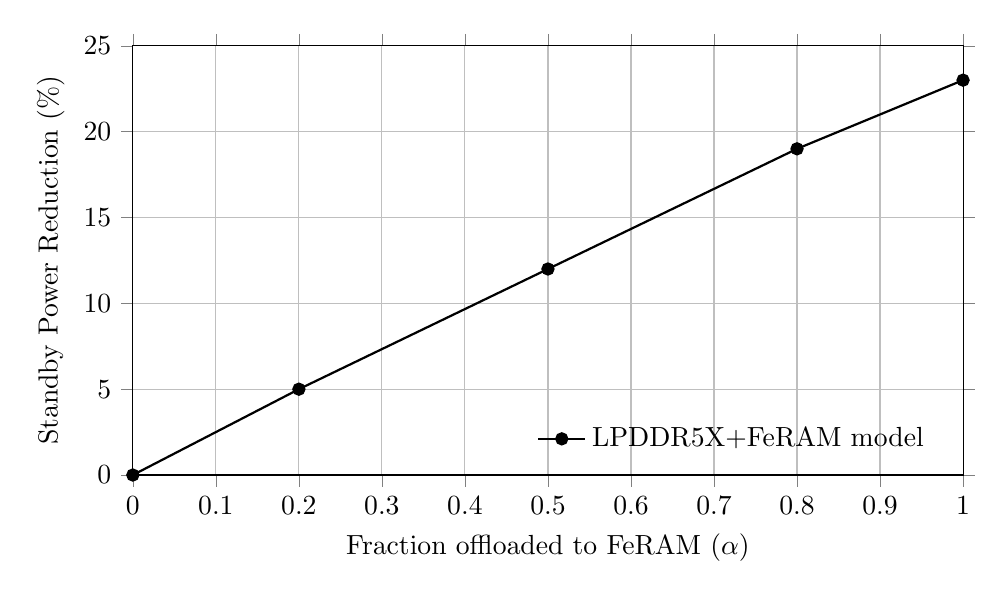
\begin{tikzpicture}
    \begin{axis}[
      width=\columnwidth,
      height=0.58\columnwidth,
      xlabel={Fraction offloaded to FeRAM ($\alpha$)},
      ylabel={Standby Power Reduction (\%)},
      xmin=0, xmax=1, ymin=0, ymax=25,
      grid=both, tick align=outside,
      legend style={at={(0.97,0.03)},anchor=south east,draw=none,fill=none}
    ]
      \addplot[thick, mark=*] coordinates {(0,0) (0.2,5) (0.5,12) (0.8,19) (1.0,23)};
      \legend{LPDDR5X+FeRAM model}
    \end{axis}
  \end{tikzpicture}
  \vspace{-1ex}
  \caption{Standby power reduction versus offload fraction $\alpha$.}
  \label{fig:standby_reduction}
\end{figure}

\subsection{Resume Latency}
Resume latency is the time from power-on to usable memory state.
Baseline LPDDR involves DRAM warm-up, MR restore, and page reload (ms-scale).
With FeRAM offloading, only DMA from FeRAM chiplet is required for checkpoints.
For 1--10~MB checkpoints and 5--10~GB/s DMA bandwidth, latency becomes 100--500~$\mu$s.

\subsection{System-Level Efficiency}
\begin{table}[t]
  \centering
  \caption{System-level efficiency impact of LPDDR+FeRAM integration.}
  \label{tab:sys_efficiency}
  \small
  \setlength{\tabcolsep}{4pt}
  \resizebox{\columnwidth}{!}{%
    \begin{tabular}{@{}lcc@{}}
      \toprule
      Metric & Baseline (LPDDR only) & LPDDR+FeRAM \\
      \midrule
      Standby power & 100\% & 80--88\% \\
      Resume latency & ms order & 100--500~$\mu$s \\
      Data retention & volatile (32--64~ms) & years (FeRAM) \\
      Effective energy efficiency & 1.0$\times$ & 1.15--1.25$\times$ \\
      \bottomrule
    \end{tabular}
  }
  \vspace{-1.0mm}
\end{table}

\subsection{Discussion}
FeRAM does not replace LPDDR; it \emph{assists} by eliminating refresh on cold regions and enabling instant resume.
Even small-capacity FeRAM (a few MB) is effective since only checkpoints and cold pages are migrated.
